\chapter{Legami}

Per raggiungere la configurazione più stabile, che corrisponde a quella dei gas nobili ($s^2p^6$), gli atomi condividono o scambiano elettroni attraverso quelli che prendenono il nome di legami. 

Esistono 3 tipi di legami chimici

\begin{itemize}
    \item legame ionico: attrazione elettrostatica tra ioni di segno opposto
    \item legame covalente: compartecipazione di elettroni tra due atomi 
    \item legame metallico: compartecipazione di elettroni tra un gran numero di atomi
\end{itemize}

Gli elettroni nel guscio più esterno, coinvolti nei legami, prendono il nome di elettroni di valenza\mkeyword{elettroni di valenza}.\\

Un'importante regola empirica è la regola dell'ottetto\mkeyword{regola dell'ottetto}, formulata da Lewis nel 1917, secondo cui quando un atomo possiede il livello elettronico esterno completo (detto guscio di valenza), in genere costituito da 8 elettroni, esso è in una particolare condizione di stabilità energetica e tende a non formare ulteriori legami. 

\section{Legame ionico}

Il modo più semplice per conseguire la configurazione a ottetto consiste nel trasferimento completo di uno o più elettroni da un atomo all'altro, con formazione di ioni di carica opposta che si attraggono elettrostaticamente: si parla in tal caso di legame ionico\mkeyword{legame ionico}. 
Esso si instaura fra elementi di elettronegatività assai diversa, tipicamente un metallo e un non metallo, come nella formazione del cloruro di sodio

\begin{equation}
    Na_{(s)} + \frac{1}{2} Cl_{2(g)} \longrightarrow NaCl_{(s)}
    \label{eq:formazione_nacl}
\end{equation}

Va osservato che la formazione degli ioni isolati allo stato gassoso è nel complesso endotermica, poiché l'affinità elettronica del cloro non compensa l'energia di ionizzazione del sodio. Il processo complessivo risulta esotermico soltanto grazie al successivo impacchettamento degli ioni nel reticolo cristallino, che libera una quantità di energia assai maggiore.\\

Non esiste dunque una molecola di $NaCl$: il composto è costituito da un reticolo tridimensionale nel quale ciascuno ione $Na^+$ è circondato da sei ioni $Cl^-$ e viceversa, secondo la disposizione più compatta possibile. 
La formula chimica esprime pertanto un rapporto stechiometrico e non un'entità discreta.\\

Si definisce energia reticolare\mkeyword{energia reticolare} l'energia richiesta per separare una mole di composto ionico solido negli ioni corrispondenti allo stato gassoso.


L'energia reticolare dipende dalla carica e dalle dimensioni degli ioni: cresce al crescere delle cariche, che compaiono come prodotto, e al diminuire della distanza interionica.\\

\subsection{Costante di Madelung}

Per ricavarne l'espressione si consideri dapprima un reticolo unidimensionale di ioni alternati a distanza $r_0$. 

\begin{figure}[h]
  \centering
  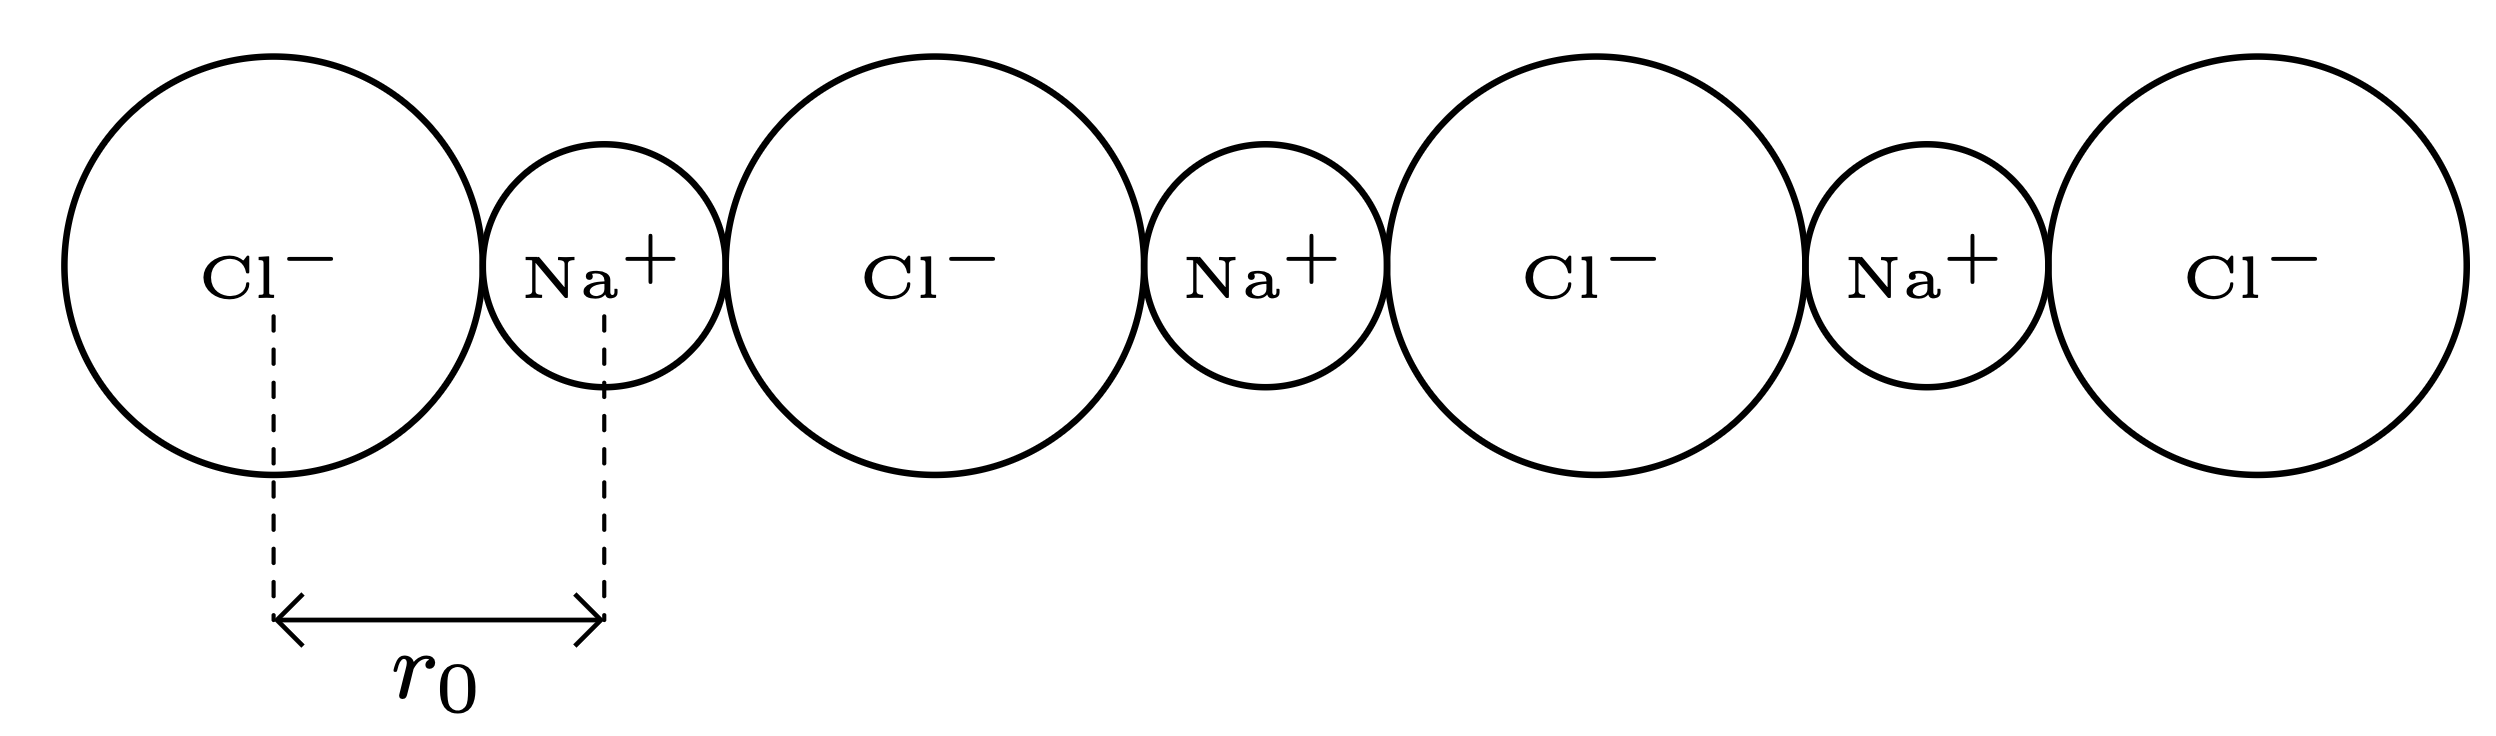
\includegraphics[width=0.7\linewidth]{foto/reticolo_1D.png}
  \caption{reticolo 1D}
  \label{fig:etichetta}
\end{figure}

Sommando i contributi coulombiani di tutti gli ioni si ottiene una serie a segni alterni, il cui valore conduce a

\begin{equation}
    E = - \frac{z_1 z_2 e^2}{4\pi\varepsilon_0 r_0} \cdot 2\ln 2
    \label{eq:madelung_1d}
\end{equation}

Nel caso tridimensionale la somma dipende dalla particolare geometria del reticolo e non è esprimibile in forma chiusa; si scrive allora

\begin{equation}
    E = - \frac{z_1 z_2 e^2}{4\pi\varepsilon_0 r_0} \cdot M
    \label{eq:madelung_3d}
\end{equation}

dove $M$ prende il nome di costante di Madelung\mkeyword{costante di Madelung} e dipende esclusivamente dalla disposizione geometrica degli ioni. Per il cloruro di sodio si ha $M = 1,7476$.\\

Il modello puramente elettrostatico descritto dalla \eqref{eq:madelung_3d} non è tuttavia completo: essendo l'energia proporzionale a $-1/r_0$, esso prevedrebbe un collasso del reticolo su sé stesso. 
Occorre aggiungere un termine repulsivo a corto raggio, di origine quantistica e riconducibile al principio di esclusione, che si oppone alla compenetrazione delle nubi elettroniche e determina la distanza di equilibrio $r_0$.\\

Le proprietà macroscopiche dei composti ionici discendono direttamente da questa struttura. Essi sono altofondenti, poiché fondere il cristallo richiede di vincere l'intera energia reticolare, e sono isolanti allo stato solido, dove gli ioni sono vincolati alle rispettive posizioni, mentre conducono la corrente se fusi o disciolti in acqua, condizioni nelle quali gli ioni acquistano libertà di movimento. Sono infine fragili: una sollecitazione esterna che faccia scorrere un piano reticolare rispetto all'adiacente porta a contatto ioni di carica uguale, e la repulsione che ne consegue provoca la frattura netta del cristallo.\\
